\documentclass[dvipsnames,tikz]{standalone}
\usepackage{amsmath}
\usepackage{arevmath}
\usepackage{xcolor}
\usepackage{tikz}
\usetikzlibrary{calc}
\usetikzlibrary{decorations.pathreplacing,calligraphy,3d}
\usetikzlibrary{lindenmayersystems}

\tikzset{main/.style={draw=black, circle, color=black}}

\begin{document}
	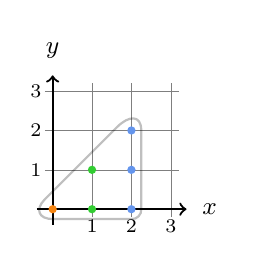
\begin{tikzpicture}[font=\small, tl/.style = {black, inner sep=1pt, font=\scriptsize} ]
		
		\draw[black!50, semitransparent, thick, xscale=-1, xshift=-1cm] (-0.125,0) to[bend right=50] (0,-0.125) -- (1, -.125) to[out=0, in=-45,looseness=1.7] (1.1,0.125) to ++(135:1.3) to[out=135, in=90, looseness=1.7] (-0.125,1) -- cycle;
		% grid
		\draw[main, very thin, xstep=0.5, ystep=0.5, semitransparent] (-0.1,-0.1) grid (1.6,1.6);
		
		% y tick label
		\foreach \y in {1, 2, 3}{
			\node[tl,left=1mm] at (0,0.5*\y) {$\y$};
		}
		% x tick label
		\foreach \x in {1, 2, 3}{
			\node[tl,below=1mm] at (0.5*\x,0) {$\x$};
		}
		
	
		% axes
		\draw[main, ->,thick] (-0.2,0) -- (1.7,0) node[right] {$x$};
		\draw[main, ->,thick] (0,-0.2) -- (0, 1.7) node[above] {$y$};	
		
		\fill[BurntOrange] (0,0) circle (1.5pt);
		\fill[LimeGreen] (0.5,0.5) circle (1.5pt);
		\fill[CornflowerBlue] (1,1) circle (1.5pt);
		\fill[LimeGreen] (0.5,0) circle (1.5pt);
		\fill[CornflowerBlue] (1,0.5) circle (1.5pt);
		\fill[CornflowerBlue] (1,0) circle (1.5pt);
		
	\end{tikzpicture}
\end{document}